\chapter{Refactoring}
\label{ch:refactoring}
El refactoring del c\'odigo original se realiz\'o en Python en su versi\'on 3.6.6 (versi\'on diferente a la que el programa fue implementado inicialmente: 2.7). Adem\'as se mantuvieron casi la totalidad de las librer\'ias cambiando \'unicamente Pymorph\footnote{\url{https://pythonhosted.org/pymorph/}} por Mahotas\footnote{\url{https://mahotas.readthedocs.io/en/latest/}} (ambas librer\'ias desarrolladas por el mismo autor, Luis P. Coelho\footnote{\url{https://github.com/luispedro}}), debido a que la primera dej\'o de ser mantenida desde el 2010 y contempla adaptaci\'on para Python 3.   

%\section{Ejecuci\'on de la rutina}
\section{Manejo de datos de entrada}
Toda las im\'agenes de entrada son manipuladas y servidas por la clase \textsc{DataPicker}. Esta clase se inicializa recibiendo un path hacia un archivo de configuraci\'on (ver Ap\'endice \ref{subs:a1}) que contiene tanto las rutas a los archivos as\'i como los nombres de estos en t\'erminos de expresiones regulares, semestre a los que corresponde la secuencia de observaciones (los dos \'ultimos d\'igitos del a\~no concatenados con la letra A en caso de corresponder al primer semestre o B al segundo), el campo (representado como un n\'umero de dos d\'igitos, comenzando con cero para valores menores a 10) y el detector CCD (cadena de tres car\'acteres donde el primero de ellos describe a que grupo de detectores corresponde: N o S (ver figura \ref{fig:f4}); adem\'as de un n\'umero entero que va de 1 a 36) como strings. 
\bigskip

El archivo que esta clase consume, para la configuraci\'on de las rutas, debe contener los siguientes campos (ver ejemplo \ref{subs:a1}).
\begin{itemize}
\item \textbf{\texttt{maskDir}}: Directorio donde se almacenan las im\'agenes m\'ascara (im\'agenes que identifican p\'ixeles que no deben ser considerados).
\item \textbf{\texttt{scienceDir}}: Directorio donde se almacenan las im\'agenes cient\'ificas (im\'agenes base ya preprocesadas).
\item \textbf{\texttt{diffDir}}: Directorio donde se almacenan las im\'agenes de diferencia (resta entre las im\'agenes base y su cient\'ifica).
\item \textbf{\texttt{psfDir}}: Directorio donde se encuentran los modelos de psf (ap\'endice \ref{a1:psf}) usados para la determinaci\'on del flujo.
\item \textbf{\texttt{invDir}}: Directorio que guarda las im\'agenes correspondientes a la varianza inversa (\textit{peso} de cada pixel en t\'erminos de ruido: a menor peso, mayor ruido).
\item \textbf{\texttt{afluxDir}}: Directorio que contiene los archivos de extensi\'on \texttt{NPY} dentro de los cuales se guarda el valor de la variable \texttt{aflux}.
\item \textbf{\texttt{maskRegEx}}: Expresi\'on regular con la que es posible identificar el nombre de las im\'agenes m\'ascara en disco siguiendo el path \texttt{maskDir}.
\item \textbf{\texttt{scienceRegEx}}: Expresi\'on regular con la que es posible identificar el el nombre de las im\'agenes cient\'ificas en disco siguiendo el path \texttt{scienceDir}.
\item \textbf{\texttt{diffRegEx}}: Expresi\'on regular con la que se identifican el nombre de las im\'agenes de diferencia en disco siguiendo el path \texttt{diffDir}.
\item \textbf{\texttt{invRegEx}}: Expresi\'on regular con la que es posible identificar el nombre de las im\'agenes de la varianza inversa siguiendo el path \texttt{invDir}.
\item \textbf{\texttt{afluxRegEx}}: Expresi\'on regular con la que se identifica el nombre de los archivos \textit{match} que contienen el valor de \texttt{aflux}. Estos archivos est\'an ubicados en el path \texttt{afluxDir}.
\item \textbf{\texttt{psfRegEx}}: Expresi\'on regular que describe el nombre de las im\'agenes que guardan el modelo de PSF en el directorio \texttt{psfDir}.
\end{itemize}


\textsc{DataPicker} maneja  la lectura y preparaci\'on de las im\'agenes a ser analizadas, mientras que un segundo proceso correspondiente a la lectura de resultados anteriores (guardados en un archivo de texto plano) se describir\'a en el Cap\'itulo 5 de nuevas funcionalidades \ref{ch:news}. 
\bigskip
  
\subsection{Lectura y preparaci\'on de im\'agenes}
A continuaci\'on se enumeran los diferentes m\'etodos que intervienen en la recolecci\'on de los datos a ser le\'idos:

\begin{itemize}
\item \textbf{\texttt{config\_reg\_expressions(semester, field, ccd)}}\\
Este m\'etodo recibe como par\'ametros el semestre (\texttt{semester}), el campo (\texttt{field}) y el ccd que la misma clase recibe de entrada. Con estos strings se establecen las rutas de los directorios de las im\'agenes y las expresiones regulares de los nombres de las mismas.
\bigskip

\item \textbf{\texttt{collect\_data()}}\\
Esta funci\'on se encarga de recolectar la ruta completa de las diferentes im\'agenes (m\'ascarac, cient\'ificas, de diferencia, etc.). Para esta finalidad se hace uso del m\'etodo \texttt{walking\_through\_files}. 
\bigskip

\item \textbf{\texttt{walking\_through\_files(regex, dir)}}\\
M\'etodo con el cual se recorren las rutas definidas en los pasos anteriores y se agrupan los nombres completos (directorio incluido) de las im\'agenes ubicadas en el directorio \texttt{dir} y posean un nombre de patr\'on que siga la expresi\'on regular \texttt{regex}.
\bigskip

\item \textbf{\texttt{filter\_science\_images()}}\\
Filtra im\'agenes cient\'ificas de acuerdo a su airmass \ref{ap:airmass}, seleccionando las fechas en que las observaciones fueron hechas en t\'erminos de \textit{d\'ia juliano modificado} o \textit{Modified Julian Date} (MJD) como variables de punto flotante.
\bigskip

\item \textbf{\texttt{select\_fits(dir)}}\\
Selecciona y ordena los elementos de la lista de im\'agenes de formato fits del directorio \texttt{dir} en orden cronol\'ogico (i.e. de acuerdo a la secuencia de MJD encontrada en \texttt{filter\_science\_images()}).
\bigskip

\item \textbf{\texttt{select\_npys(dir, ref\_dir, init\_index, n\_pos, rest\_len)}}:\\
Selecciona los archivos de extensi\'on NPY que se encuentran en el directorio \texttt{dir}. Los nombres son filtrados en relaci\'on a las im\'agenes listadas de \texttt{ref\_dir} seg\'un el paso de \texttt{select\_fits(dir)} (es decir, debe ser un directorio que contenga im\'agenes FITS). \texttt{init\_index}, \texttt{n\_pos} y \texttt{rest\_len} son enteros usados para extraer substrings espec\'ificos de los nombres de los archivos.
\end{itemize}

\section{Determinaci\'on de flujos}
El proceso de la obtenci\'on del flujo se simplific\'o, eliminando la clase FitsHandler del programa original. Debido a la posibilidad de hacer los m\'etodos de esta clase est\'aticos se implement\'o un script Python denominada \texttt{utils} para contener estas rutinas e implementarlas est\'aticamente.
\bigskip

Los m\'etodos que participan en la rutina de calculo de flujo son: 

\begin{itemize}
\item \textbf{\texttt{naylor\_photometry(invvar, diff, psf)}\cite{naylor}:}\\
Calcula el producto del flujo por su variaza. Retorna el producto y la varianza. Para esto obtiene el flujo a partir de la imagen PSF entregada (\texttt{psf}) y del producto entre la imagen diferencia y la de varianza inverza (\texttt{diff} y \texttt{invvar} respectivamente).
\bigskip


\item \textbf{\texttt{calc\_fluxes(diff, psf, invvar, aflux)}:}
Calcula el flujo y su varianza gestionando la entrada y la salida de \texttt{naylor\_photometry(invvar, diff, psf)}. Los valores NaN son transformados a valores de punto flotante de constante 0.001.
\end{itemize} 

Estos m\'etodos  son llamados desde la rutina \textsc{RoutineHandler} (ver en el cap\'itulo \ref{ch:news}).
\section{Filtros originales}
La refactorizaci\'on de los filtros de Kalman originales implic\'o la implementaci\'on de nuevas clases e interfaces para el desarrollo del patr\'on propuesto: Strategy. A continuaci\'on se presentan cada una de ellas:

\begin{itemize}
\item \textbf{IPredict:} Interface que describe el comportamiento de la funci\'on \textsc{Predict} de un filtro de Kalman. \texttt{predict} recibe como par\'ametros el paso de tiempo ($\Delta t$), la matriz de estado, la matriz de covarianza de estado, y las predicciones de las matrices de estado y covariaza determinadas en el paso anterior (con la finalidad de actualizar estas variables). Su firma queda como:
\begin{center}
\texttt{predict(delta\_t, state, state\_cov, pred\_state, pred\_cov)}
\end{center}
Este m\'etodo entrega finalmente las matrices de estado y covarianza de estado predicho.
\bigskip

\item \textbf{ICorrect:} Interface que describe el comportamiento de la funci\'on \textsc{Correct} de un filtro de Kalman. \texttt{correct} recibe como par\'ametros el matriz de flujo (\texttt{z}) y de varianza de las observaciones (\texttt{R}), la matriz de estado predicha, la matriz de covarianza predicha, la matriz de estado y la matriz de covarianza (para sobreescritura) obtenidas en el paso anterior. Su firma queda como:
\begin{center}
\texttt{correct(z, R, pred\_state, pred\_cov, state, state\_cov)}
\end{center}
\bigskip
Esta funci\'on entrega finalmente las matrices de estado y covarianza de estado corregido.

\end{itemize}

\subsection{Strategies de predicci\'on}
\textbf{LinearPredict:} Clase que extiende de IPredict. Implementa m\'etodo \texttt{predict} que ser\'a usado tanto por el filtro b\'asico como el de m\'axima correntrop\'ia. Su instanciaci\'on recibe como argumento \texttt{sigma\_a} (desviaci\'on est\'andar del modelo, asumiendo una distribui\'on gaussiana en la distribuci\'on de las observaciones).
\bigskip


\subsection{Strategies de correcci\'on}
\textbf{BasicCorrect:} Clase que extiende de ICorrect. Implementa m\'etodo \texttt{correct} que ser\'a usado para el tipo de filtro de Kalman B\'asico.
\bigskip

\textbf{MCCorrect:} Clase que extiende de ICorrect. Implementa m\'etodo \texttt{correct} que ser\'a usado para el tipo de filtro de Kalman de m\'axima correntrop\'ia. El constructor de esta clase recibe los siguientes par\'ametros:

\begin{itemize}
\item \texttt{epsilon}: Cantidad con la cual se contrastar\'a el error o precisi\'on que se quiera lograr con la estimaci\'on.
\item \texttt{max\_iter}: N\'umero m\'aximo de iteraciones.
\item \texttt{silverman}: \textit{boolean}. Determina si se usa o no la apoximaci\'on de Silverman para la desviaci\'on estandar.
\item \texttt{std\_factor}: Factor de desviaci\'on est\'andar usado en la aproximaci\'on de Silverman.
\item \texttt{sigma}: Sigma usado para el kernel Mercer.
\end{itemize}

\subsection{Filtros refactorizados}

\begin{itemize}
\item \textbf{KalmanFilter:} Clase abstracta padre de los subtipos BasicKalmanFilter y MCKalmanFilter. Posee los m\'etodos abstractos \texttt{predict} y \texttt{correct}, que son definidos de acuerdo a las estrategias de predicci\'on y correci\'on descritas previamente.
\item \textbf{BasicKalmanFilter:} Representa el filtro b\'asico de Kalman. Est\'a compuesto por las estrategias \texttt{LinearPredict} y \texttt{BasicCorrect}.
\item \textbf{MCKalmanFilter:} Representa el filtro de m\'axima correntrop\'ia. Est\'a compuesto por las estrategias \texttt{LinearPredict} y \texttt{MCCorrect}.
\end{itemize}
\bigskip

\begin{figure}
\centering
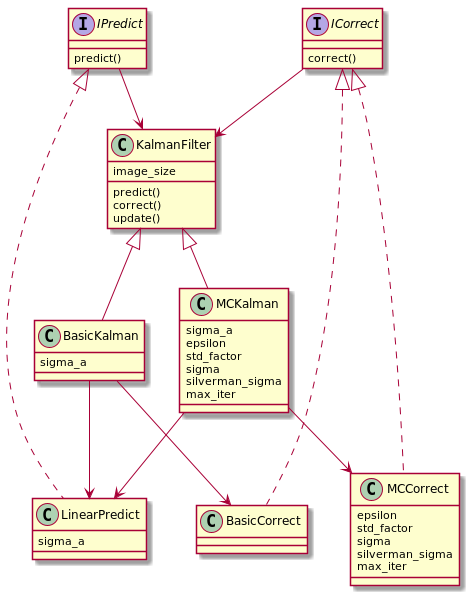
\includegraphics[scale=.5]{images/kalmanfilter_class}
\caption{Familia de filtros de Kalman y patr\'on strategy usado en la implementaci\'on de los m\'etodos \texttt{predict} y \texttt{correct}.}
\label{fig:ref1}
\end{figure}

\section{Detecci\'on de candidatos}
La detecci\'on de candidatos en el programa original se realiza en \textsc{SNDetector} sin embargo, durante este refactoring se descompuso el proceso de reconcimiento de fuentes estelares (grupo de pixeles brillantes) del proceso de selecci\'on de candidatos, siendo este la continuaci\'on del primero. Por tanto se crearon las clases \textsc{SourceFinder} para el filtrado y agrupamiento de pixeles y \textsc{TPDetector} (transient phenomena detector) para la revisi\'on de las \textit{fuentes} encontradas en el paso anterior.
\subsection{SourceFinder}
La clase \textsc{SourceFinder} posee los siguientes m\'etodos:
\begin{itemize}
\item \texttt{pixel\_discard}:\\
M\'etodo en el que se realiza el descarte de pixeles de forma individual, siguiendo los siguientes criterios:
\begin{enumerate}
\item Si el estado (flujo) calculado para un pixel es menor que el umbral dado.
\item Si la tasa de cambio estado (cambio o variaci\'on de flujo) es menor que el umbral de variaci\'on de flujo multiplicado por el nivel de saturaci\'on alcanzado en esta variaci\'on (se define una tasa de saturaci\'on \textit{aceptable}).
\item Si un pixel de la imagen cient\'ifica es menor a la mediana m\'as un valor arbitrario (en este trabajo, siguiendo la l\'inea de desarrollo de P. Huentelemu, se consider\'o 5.0) es descartado.
\item Si las varianzas de flujo son mayores a 150.0 (valor arbitrario).
\item Si las varianzas de la tasa de cambio de flujo (o velocidad de flujo) es mayor o igual a 150.0.
\item Si los pixeles no caen en etiquetas de invalidaci\'on dentro de la m\'ascara que ha sido procesada para marcar tambi\'en los pixeles vecinos a los realmente defectuosos.
\item Si los pixeles no han ca\'ido dentro del descarte por superar la mediana estiamda a partir de cuatro \'epocas. 
\end{enumerate}
\item \texttt{grouping\_pixels(pixel\_flags, mjd\_index)}:\\
Este m\'etodo recibe como entradas las etiquetas determinadas en el paso anterior en un arreglo de matrices (\texttt{numpy array}) denominado \texttt{pixel\_flags}. Adem\'as recibe el \'indice de MJD (o fecha en d\'ia juliano modificado) correspondiente a la observaci\'on de tal fecha.
La agrupaci\'on de pixeles se realiza gracias a funciones brindadas por la librer\'ia \textsf{Mahotas}, usando el m\'etodo \texttt{label} para encontrar dominios cerrados en el mapa de pixeles validados.
\bigskip

\item \texttt{filter\_groups(science, flux, var\_flux, state, base\_mask, median\_reject)}:\\
Este m\'etodo recibe la imagen cient\'ifica, el flujo y su varianza, el estado determinado por el filtro de Kalman, la m\'ascara, y un arreglo en el que se guardan los valores de las medianas por cada cuatro observaciones. 
El filtrado de grupos de pixeles se lleva a cabo bajo las siguientes reglas de descarte: 

\begin{enumerate}
\item Descarte de grupo por contener posible mala resta alrededor (valores negativos).  
\item	Si no hay m\'aximos locales dentro del grupo de pixeles encontrados dentro de la imagen cient\'ifica.
\item	Si no hay m\'aximos locales dentro del grupo de pixeles encontrados dentro de la matriz de flujo.
\item	Si no hay m\'aximos locales dentro del grupo de pixeles encontrados dentro de la matriz velocidad de flujo.
\item 	Si los valores de los pixeles superan la mediana local en imagen cient\'ifica.
\item	Si el grupo posee alg\'un pixel que doble el valor del flujo o de la imagen cient\'ifica.
\item	Si el centro del grupo se encuentra etiquetado como defectuoso dentro de la m\'ascara.
\item	Si el pixel del centro del grupo se encuentra rechazado al ser superior a la mediana de los pixeles de cuatro observaciones consecutivas.
\item	Si la varianza del flujo del pixel del centro del grupo es mayor al determinado por el umbral.
\end{enumerate} 
\item \texttt{draw\_complying\_pixel\_groups}:\\
Este m\'etodo es el que llama a \texttt{pixel\_discard} para etiquetar pixeles para el descarte y no ser considerados posteriormente en el paso de agrupamiento al llamar a \texttt{grouping\_pixels}. Luego se llama al m\'etodo \texttt{filter\_groups} para hacer el descarte a nivel grupal y obtener candidatos. La \'ultima llamada es para el m\'etodo \texttt{save\_data} que se encuentra en clase \textsc{DataContent}. 
\end{itemize}

\section{Visualizaci\'on de resultados}
La visualizaci\'on de los resultados se realiza a trav\'es de la clase \textbf{Visualizer} con el cual se generan dos diferentes gr\'aficas usando la librer\'ia \textsc{MatplotLib}. 
\begin{itemize}
\item \textbf{Curvas de flujo observado, estimado y predicho, con sus respectivas varianzas}. Otorga informaci\'on del comportamiento de los flujos de inter\'es durante las diferentes \'epocas (medidas en MJD). 
\item \textbf{Estampillas}. Se muestra el comportamiento del flujo a trav\'es de los pixeles de diferentes matrices: imagen cient\'ifica, PSF, flujos observado y su varianza, estados de flujo y su velocidad estimados, etiquetas de pixeles y de grupos de pixeles.
\end{itemize}

Estas gr\'aficas son generadas gracias a los siguientes m\'etodos:

\begin{itemize}
\item \texttt{plot\_lightcurve(coords, position, filename):}\\
M\'etodo destinado a crear la serie de curvas de flujo observado, estimado y predicho junto con sus respectivas velocidades de flujo (estimado, predicho) y varianzas. La variable \texttt{coords} corresponde a la coordenada del objeto estudiado en la primera imagen cient\'ifica. La variable \texttt{position} guarda la posici\'on del mismo objeto en las estampillas (se asume la misma posici\'on ya que est\'an alineadas). Por \'ultimo, \texttt{filename} corresponde al nombre del archivo con el que se va a guardar la imagen resultante (de extensi\'on PNG, por convenci\'on).  
\item \texttt{print\_stamps(coords, filename):}
Recibe el nombre del archivo con el cual se guardar\'a la imagen. Es la funci\'on encargada de construir la imagen donde se muestra la evoluci\'on de los flujos y las etiquetas de los pixeles en diferentes etapas en las estampillas obtenidas previamente.
\end{itemize}

\begin{figure}
\centering
\includegraphics[scale=.3]{/home/paloma/Documents/Memoria/Code/sif2/sif/resultsplots/FN/par-00_HiTS14_SN-nay_3278-1883_lightcurves.png}
\caption{Ejemplo de curva de flujo y velocidad de flujo observados, estimados y predichos, de una supernova encontrada por HiTS. }
\label{fig:lc_result}
\end{figure}

\begin{figure}
\centering
\includegraphics[scale=.3]{/home/paloma/Documents/Memoria/Code/sif2/sif/resultsplots/FN/par-00_HiTS14_SN-nay_3278-1883_stamps.png}
\caption{Estampillas de matrices de pixeles y etiquetas que muestran el comportamiento del flujo a trav\'es del tiempo: la primera fila de im\'agenes corresponde a estampillas obtenidas desde las im\'agenes cient\'ificas en donde debiese habitar la supernova observada durante todo el periodo de observaci\'on (definido por las \'epocas). La siguiente fila inferior muestra los diferentes modelos de PSF obtenidos para diferentes \'epocas. La tercera fila muestra el flujo observado en la misma posici\'on. Le sigue la varianza de este flujo. Posteriormente viene el flujo estimado por el filtro de Kalman siguiendo la velocidad de flujo estimado. Finalmente vienen las etiquetas de los pixeles reconocidos por el programa como pertenecientes a un objeto transiente (etiquetado por pixel y pot grupo de pixeles). La \'ultima fila corresponde a la m\'ascara base usada en todo el an\'alisis.}
\label{fig:lc_result}
\end{figure}
\bigskip

%El estilo de las gr\'aficas de la versi\'on refactorizada respet\'o el dise\~no original de las gr\'aficas, especificados por Pablo Huentelemu.